\documentclass{beamer}
\usepackage[utf8]{inputenc}
\usepackage[francais]{babel}
\usepackage[T1]{fontenc}
%\usepackage{multimedia}
\usepackage{graphicx}
\usepackage{hyperref}
\usepackage{algorithm}
\usepackage{algpseudocode}
\floatname{algorithm}{Algorithme} 

%\usetheme[width=100pt]{PaloAlto}
\usetheme{Ilmenau}

%\setbeamercovered{transparent}

\title{Proactive : an Open Source Middleware for parallel computing}

\author{Veyssier Julien}
\institute{CBGP- INRA}
\date\today
\setbeamertemplate{navigation symbols}{}
%\logo{}
\begin{document}

\begin{frame}
\titlepage
\end{frame}

\begin{frame}
\tableofcontents
\end{frame}

\section[Introduction]{Introduction}
\begin{frame}
	\tableofcontents[currentsection]
\end{frame}

\begin{frame}{DIYABC}
	\begin{columns}
	\begin{column}[l]{0.5\linewidth}
        \begin{figure}
            %[!bh]
            \centering
            
\includegraphics[scale=0.39]{cbgp.png}
            %\caption{Architecture autour d'un CDN}
        \end{figure}
        \begin{figure}
            %[!bh]
            \centering
            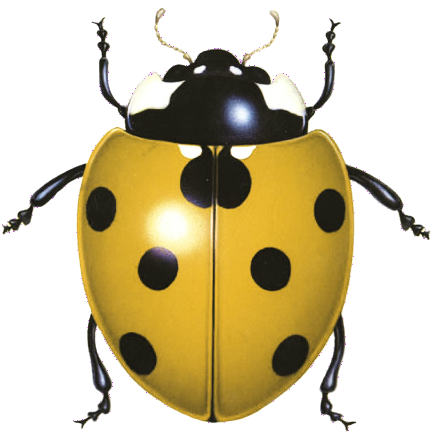
\includegraphics[scale=0.39]{cocci.png}
            %\caption{Architecture autour d'un CDN}
        \end{figure}

	\end{column}
	\begin{column}[r]{0.5\linewidth}
	\begin{block}{}
			\begin{itemize}
				\item Implémentation de l'interface graphique
                \item 
			\end{itemize}
					
		\end{block}
	\end{column}
	\end{columns}
\end{frame}

\begin{frame}{CDN et P2P}
    plap
\end{frame}



\begin{frame}
	%TODO schema qui illustre lincoherence entre topologies
	\begin{columns}
		\begin{column}[l]{0.65\linewidth}
	\begin{block}{Concepts}<1->
		\begin{itemize}
			\item CDN
			\item P2P (Peer to Peer) % passage à lechelle ->
			            		%good for CDN
			\item Routage logique
			\item Routage physique
		\end{itemize}
	\end{block}
	\begin{alertblock}{Objectif}<2->
		Optimiser le routage en se concentrant sur les différences
		entre topologie logique et physique
	\end{alertblock}
	\end{column}

		\begin{column}[r]{0.35\linewidth}
            blurp
\end{column}
\end{columns}
\end{frame}

\section[Fonctionnement]{Fonctionnement de Proactive}
\begin{frame}
	\tableofcontents[currentsection]
\end{frame}

\begin{frame}
	% constat, propo, exemple

		\begin{block}{Travail effectué}<1->
		\begin{itemize}
			\item Constat%diff entre topos
			\item Propositions
			\item Étude d'un exemple d'application
		\end{itemize}
		\end{block}

		\begin{exampleblock}{Perspectives}<2->
		\begin{itemize}
			\item Établir une norme sur les échanges de messages
				%pour favoriser les
				%reflexions sur ce genre d'opti?
			\item Cache s\'electif (images, degr\'e de volatilit\'e)
			\item Élaboration de protocoles applicatifs pour la
				communication entre routeurs (Gossiping)
			\item Création d'une architecture spécialisée pour les CDN
			\item Proposition d'extension du protocole IP proposant
				des primitives de plus haut niveau dans les
				routeurs
		\end{itemize}
		\end{exampleblock}
	% 
\end{frame}

\begin{frame}
	\begin{center}	{\huge Merci de votre attention}\end{center}
	\end{frame}
\begin{frame}
	\begin{center}	{\huge Questions}\end{center}
	\end{frame}

\end{document}
